\documentclass{article}
\usepackage[utf8]{inputenc}
\usepackage[T1]{fontenc}
\usepackage[british]{babel}
\usepackage{datetime2}
\usepackage{graphicx}
\usepackage{hyperref}
\usepackage{abstract}
\renewcommand{\abstractname}{}
\usepackage{titling}
\usepackage{caption}
\usepackage{verbatim}

\date{\today}
\pretitle{\begin{center}\LARGE}
\posttitle{\end{center}}
\title{An Intelligent Agent-Based Framework for Automated Test Case Generation from Natural Language}
\author{Alberto Espinosa\\
KSquare}

\begin{document}

\maketitle

\begin{abstract}
\noindent
This document outlines the architecture and implementation strategy for a novel intelligent agent-based system designed to automate the generation of test cases. The proposed framework addresses the inefficiency of manual test case creation by ingesting natural language test steps and converting them into executable, maintainable test scripts. The system leverages a multi-agent workflow orchestrated by a graph-based framework, such as LangGraph, and a large language model (LLM) to parse, comprehend, and generate code. This report details the functionality of each agent within the pipeline, their interdependencies, and the integration with an existing test execution and reporting system, thereby providing a comprehensive, self-contained description of the architecture.
\end{abstract}

\section{Introduction}
The development of robust and scalable software is intrinsically linked to the quality of its testing. The existing process for test case creation, as noted within the development team, is predominantly manual, leading to significant time and resource expenditure. The current system, as detailed in \texttt{notebook\_24.ipynb} (authored by QA-Project-Team), is a powerful execution engine for test artifacts, yet it lacks an automated method for generating these artifacts from high-level, human-readable specifications. This limitation hinders the team's ability to achieve broader test coverage and accelerate the continuous integration cycle. The solution proposed is to implement an intelligent pipeline that can process natural language test descriptions and automatically produce the necessary test code, effectively bridging the gap between human intent and automated execution.

\section{System Architecture}
The proposed system is architected as a sequential, multi-agent pipeline, orchestrated using a graph-based framework like LangGraph. Each agent is responsible for a specific stage of the test generation process, with the output of one agent serving as the input for the next. The system’s core is a Large Language Model (LLM) which provides the necessary intelligence for comprehension and code generation. The architecture is composed of five distinct agents, the fifth of which is the pre-existing system.

\subsection{Agent 1: The Input Agent}
The first component in the pipeline is the Input Agent. Its primary function is to ingest natural language test cases. These can be in the form of plain text files or parsed from structured data sources like images or spreadsheets. The agent processes this raw data, normalises the text, and prepares it for contextual analysis by the subsequent agent. A clear example of such a structured input is shown in Figure~\ref{fig:testcase1}, which demonstrates how test steps are documented in a human-readable format.

\begin{figure}[h!]
    \centering
    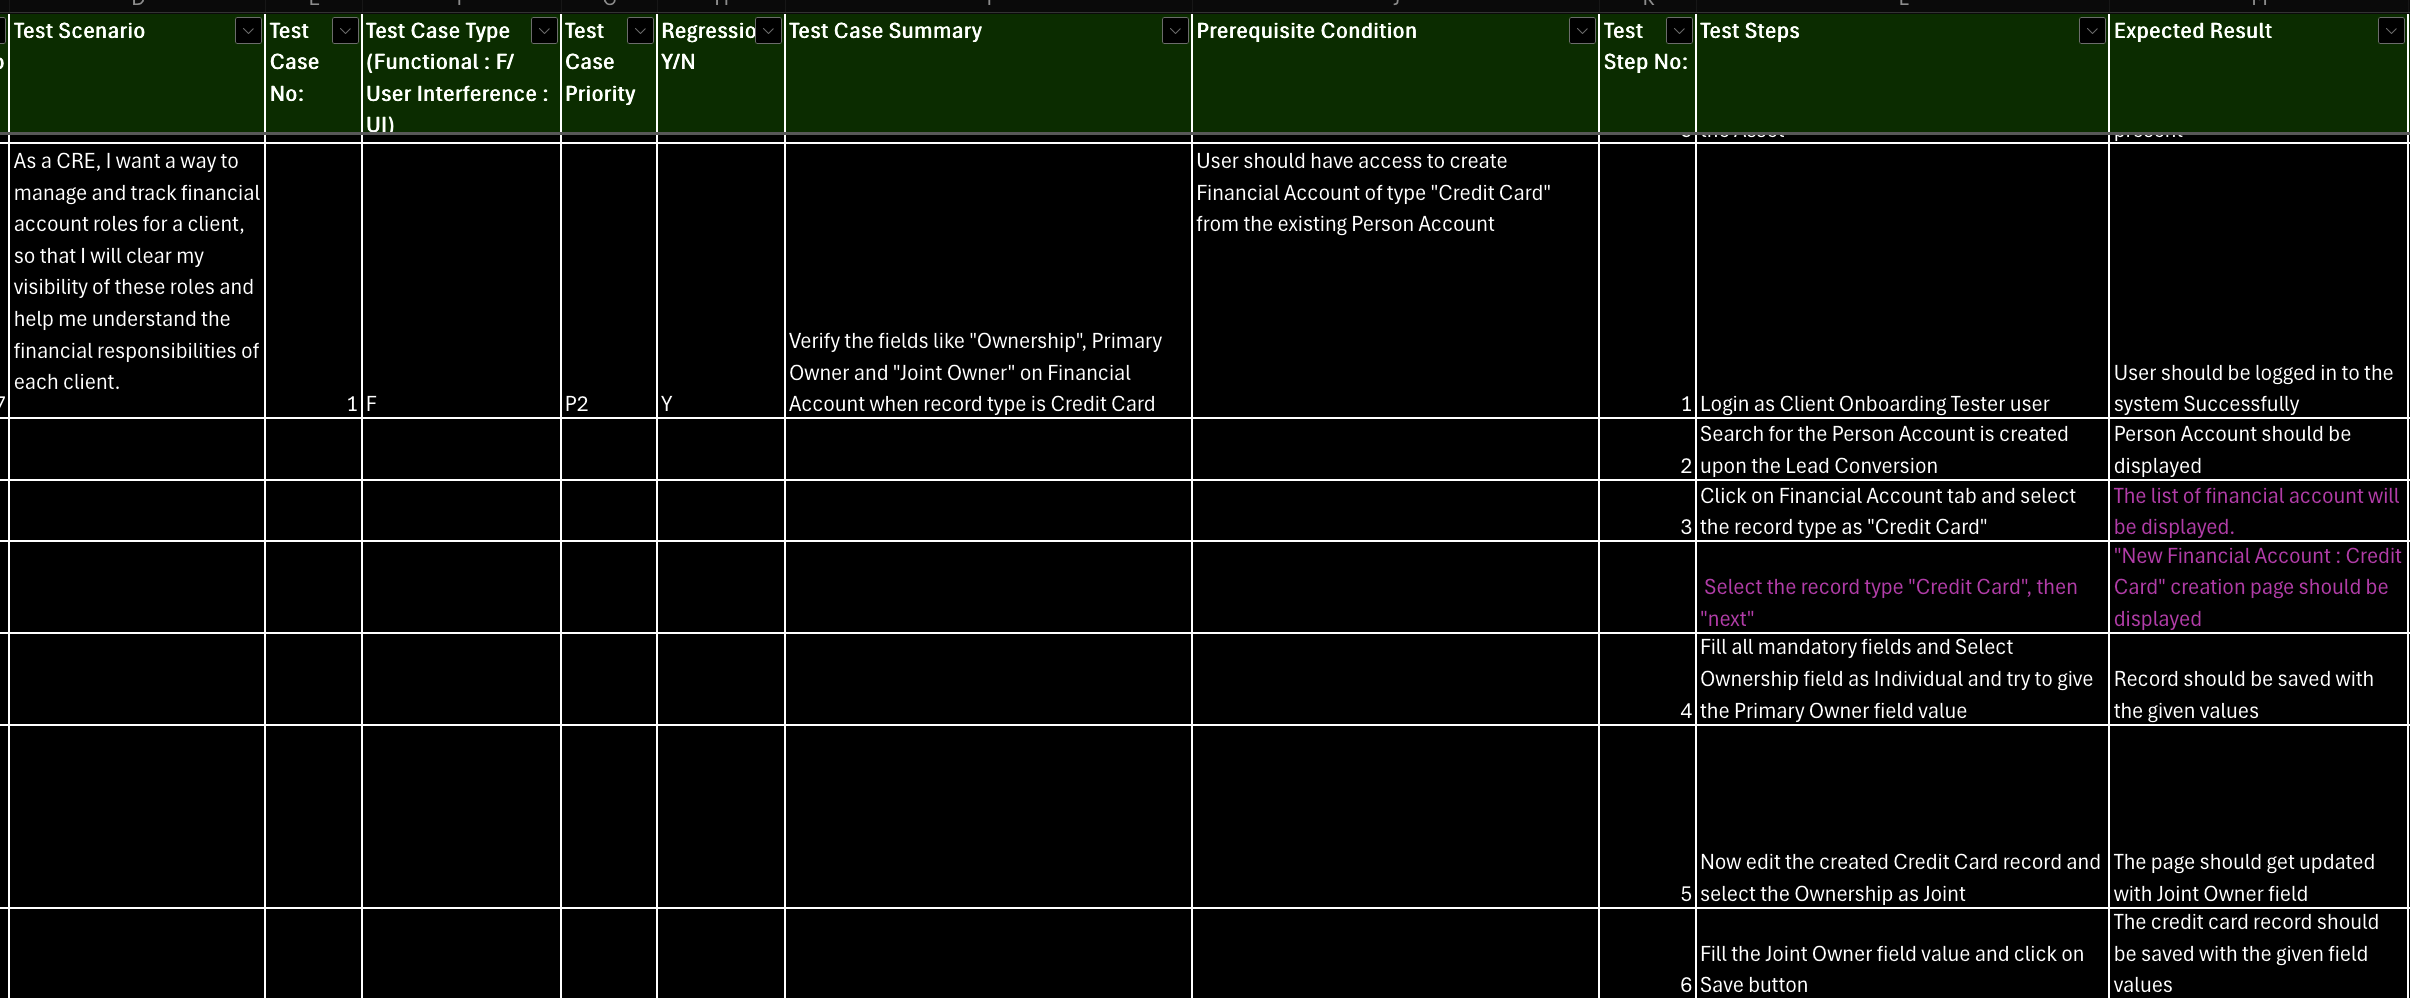
\includegraphics[width=1\textwidth]{images/testCase1.png}
    \caption{Example of a manual test case provided in natural language. The Input Agent processes this document to extract key fields like Test Case ID, Use Case, and especially the Test Steps, which contain the actions to be automated.}
    \label{fig:testcase1}
\end{figure}

\subsection{Agent 2: The Parsing and Comprehension Agent}
This is the most critical component of the new architecture. The Parsing and Comprehension Agent takes the clean, raw text from the Input Agent and uses the LLM to understand its meaning. It analyses the natural language steps to extract key entities and actions, such as:
\begin{itemize}
    \item \textbf{URLs} (e.g., ``navigate to \texttt{www.google.com}'')
    \item \textbf{User Inputs} (e.g., ``type 'Playwright' in the search bar'')
    \item \textbf{Element Identifiers} (e.g., ``the search bar,'' ``the 'Search' button'')
    \item \textbf{Expected Outcomes} (e.g., ``verify that the search results are displayed'')
\end{itemize}
The output of this agent is a structured, machine-readable representation of the test case's logic. It is important to clarify that this process does not require real-time access to the URL or the web application itself. The agent's intelligence is solely based on the textual information provided. It ``understands'' the intended actions by analysing the syntax and semantics of the text, mapping phrases like ``navigate to'' to the concept of a URL, and ``type into'' to a user input action. The system's ability to generate test code is therefore decoupled from the need to interact with a live environment, making the generation process fast and stable.

\subsection{Agent 3: The Test Plan Generation Agent}
Following comprehension, the Test Plan Generation Agent formulates a formal test plan. This component translates the structured data from the previous agent into a high-level plan for test execution. It determines the sequence of actions, defines the assertions required to validate the outcomes, and specifies the necessary setup and teardown procedures. This plan is framework-agnostic at this stage but provides the blueprint for the final code.

\subsection{Agent 4: The Code Generation Agent}
This agent is responsible for converting the high-level test plan into executable code. It uses the LLM to generate code in the target test automation framework, specifically \textbf{Playwright}. The output of this agent is a \textbf{Python script} (`.py` file) that contains the complete test code. The file is structured and organised to be immediately compatible with the existing test execution framework. Each generated test case will be a distinct function, typically organised within a class, following standard testing conventions (e.g., using \texttt{pytest}). The output includes:
\begin{itemize}
    \item Necessary imports from the Playwright library (e.g., \texttt{playwright}, \texttt{sync\_playwright}).
    \item Test setup and teardown code.
    \item A sequence of Playwright actions (e.g., \texttt{page.goto()}, \texttt{page.fill()}, \texttt{page.click()}).
    \item Assertions to validate expected outcomes (e.g., \texttt{expect(page).to\_have\_title()}).
\end{itemize}
The output's format is designed to be directly consumable by Agent 5, ensuring a seamless handover.

\subsection{Agent 5: The Execution and Reporting Agent (Existing System)}
The final step in the pipeline integrates seamlessly with the existing system, as described in \texttt{notebook\_24.ipynb}. The inputs from Agent 4---the newly generated Python test files---are treated as standard test scripts. The existing framework, which uses Playwright and likely a test runner like \texttt{pytest}, simply discovers and executes these files. The framework is already configured to run tests and collect data, so no modifications are required to this part of the system's logic. The expected outputs of this agent remain the same:
\begin{itemize}
    \item Test execution results (pass/fail status).
    \item Detailed execution logs.
    \item Code coverage reports.
    \item Generated Gherkin features, if configured.
\end{itemize}
This agent effectively closes the loop, taking the generated code and providing the concrete results needed to confirm the success of the automation process.

\section{Practical Integration and Example}
The current system, as evidenced by the provided files, already tests against a live web application. The scripts are not ``simulations'' but actual instructions for a browser automation tool. The primary value of the new four-agent pipeline lies in automating the creation of these scripts.

For instance, consider the provided test file \texttt{checkContact.cy.js}. This file was manually written to test a live website with a URL \texttt{https://www.udaykumar.tech/}. A human developer had to manually create the following Cypress test code:

\begin{verbatim}
describe("Check Contact", () => {
    it("Check Contact", () => {
        cy.visit("https://www.udaykumar.tech/")
        cy.url().should('eq', 'https://www.udaykumar.tech/')
        cy.get('input#name').type('Uday Kumar').should('have.value', 'Uday Kumar')
        cy.get('#outlined-basic').type("7670848696").should('have.value', '7670848696')
        //...
    })
})
\end{verbatim}

The existing system, Agent 5, simply takes this file and runs it. The test engine launches a browser, navigates to the specified URL, and executes each command in sequence. If the website does not contain an \texttt{input} with \texttt{id="name"}, the test fails. The notebook then logs this failure and reports it.

The new approach dramatically improves this workflow. Instead of a human performing this tedious work, the new pipeline would start with a simple description, such as: ``Given the contact page URL, enter a name, phone number, and email into the form.'' Agents 1--4 would then automatically generate a test script identical to the one above, which is then fed into Agent 5 for execution. This transformation automates the entire test creation process, allowing for the rapid scaling of test coverage without a corresponding increase in manual labour.

\section{Future Work and Enhancements}
While the proposed architecture provides an effective and scalable solution, future enhancements could introduce more sophisticated methodologies to further improve test coverage and reliability. Two notable avenues for future development are:
\begin{itemize}
    \item \textbf{Model-Based Testing (MBT):} This approach involves creating a formal model of the application's behaviour and state transitions. An algorithm could then traverse this model to generate comprehensive test cases, potentially uncovering edge cases that might not be captured in human-written descriptions. This would serve as a powerful complement to the current natural language approach.
    \item \textbf{Agentic Search with Autonomous Code Generation:} A more advanced system could feature an autonomous agent capable of browsing a website, observing its structure, and generating test cases based on user stories without any pre-existing manual test steps. This would require the agent to dynamically interact with the UI, interpret the layout, and infer user intent, representing a significant leap in autonomy.
\end{itemize}
These enhancements would build upon the foundation of the proposed system, incrementally advancing the test automation framework towards a fully autonomous state.

\section{Conclusion}
The proposed agent-based framework represents a professional and affordable solution to the current test automation challenges. By automating the conversion of natural language test cases into executable code, the system will significantly reduce manual effort, accelerate the development cycle, and improve overall test coverage. Its modular, agent-based architecture allows for incremental development and future integration of more advanced methodologies, making it a robust and scalable solution. This framework is a strategic investment that will enhance the team's capacity to deliver high-quality software with greater efficiency.

\end{document}
